% !TeX root = ../thuthesis-example.tex

\chapter{绪论}


\section{研究背景及其意义}
\subsection{社团发现}
随着信息时代的到来,人类进入了网络化的世界。绝大部分的网络均
存在一定的社团结构\cite{fortunato2010community},
比如社交网络中的圈子、流行病网络中集中爆发的区域,以及自然界中的群落以及无线蜂窝网络中的小区等。
在网络科学中,社团结构是指
具有相同特征的节点集合, 属于同一社团的节点之间连接紧密而属于不同社团节点间的连接稀疏。
而社团发现(也称为社团检测)作为网络科学研究的重点问题之一,是指通过一定的方法寻找网络中特定的社团结构,
在社会工程、生物化学、与计算机科学等领域均有着重要的应用。
比如在社会工程领域
用于划分互联网社交媒体中的用户社群\cite{6750167},以及在推荐系统设计中划分用户社团以实现精准推荐 \cite{10.1145/2739480.2754670}。
在生物化学领域用于在蛋白质分子交互作用的网络中识别特定的功能模块 \cite{ayati2015mobas}。
%研究中有助于发现特定的微观结构,
%在社会科学领域
在
计算机科学的分布式计算中需要将任务分配给不同的计算节点,
使得不同的任务之间有尽可能
小的耦合\cite{topcuoglu2002performance}。
如图\ref{fig:distributed_computing}所示,通过社团发现将
任务划分为不同的社团,可有效减少计算节点间的通信成本。

\begin{figure}[!ht]
    \centering
    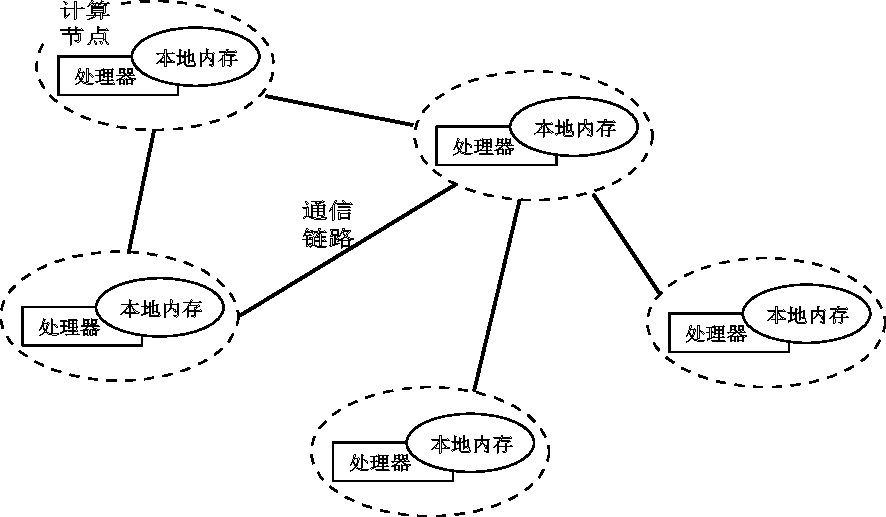
\includegraphics[width=0.6\textwidth]{background.pdf}
    \caption{分布式计算中的任务分配\protect\footnotemark}
    \label{fig:distributed_computing}
\end{figure}
\footnotetext{图片来源于网络:\url{https://medium.com/@wisnu3121/how-distributed-computing-works-3dc0c8bdef10}}

% add a paragraph to praise the existing study of community detection algorithms

社团发现的实现离不开自动化算法的支撑,伴随着计算机科学的发展,
社团发现算法的发展主要经历了三个阶段。
在本世纪以前,社团发现主要是借用解决图分割或数据聚类问题的方法,
算法复杂度较高,仅适用于小规模的网络。
得益于计算能力的提升,21世纪初十年代,以遗传算法为代表的随机优化策略在解决
各领域问题上取得了效果,结合模块度的优化目标,在此阶段涌现了大量的
社团发现算法,比较有代表性的还有标签传播和利用贝叶斯进行模型的参数估计等 \cite{fortunato2010community}。
这些算法突破了的限制,可用于求解较大规模和复杂网络,并拓展到动态图的社团发现。
10年代以来,以深度学习为代表的人工智能技术逐渐应用到社群发现问题上来,
通过从图结构的数据中学习低维表示,该类方法在有辅助信息的场景下具有更大的灵活性
\cite{Su_2022}。

%而好的社团发现算法
%需要有特定的理论支撑,以便助其在各领域实现广泛应用。

尽管社团发现领域的算法研究不断取得突破,但目前对社团发现问题的
理论认识仍较为有限,成为了制约网络科学发展的瓶颈。
在算法设计层面上,由于算法设计缺少理论指导,算法设计往往以启发式的方式进行。
尽管这些算法在准确率上更胜一筹,但在实际问题中往往要进行超参优化与
多轮迭代,既消耗了大量的计算资源,同时检测效果也不一定能得到保障。
在算法评价层面上,由于在理论层面对社团的概念缺少统一的定义,
不同算法之间难以实现公平的比较,从而给社团发现算法的选择造成了一定的困难。
在算法可靠性层面上,由于对算法的误差率缺少理论研究,
难以保证在新的问题上已有的算法能取得良好的效果。

由于网络中包含大量的节点信息和边的信息,信息论提供了度量这些信息
的有效方式,为社团发现理论研究和算法设计提供了新的思路。


\subsection{信息论度量}
信息论的概念最早由香农提出,用以解决通信领域的问题 \cite{shannon1948mathematical}。
信息论的度量如熵、互信息等是概率分布的函数,
在对信源和信道的概率化建模的基础上,
用于度量信源编码和信道传输的理论极限。此外,信息论度量在统计推断
领域也有重要的应用,如假设检验问题中的误差指数、无偏估计的理论下界等。


在通信领域的问题研究中,信息论度量的成功应用有赖于可设计的概率分布的模型。
在实际的网络中则缺少这种对分布的先验知识。这给信息论度量在社团发现问题上的应用
造成了一定的困难。目前应用信息论度量进行社团发现的相关研究克服这一困难从方法上可主要分为两大类:
其中一类是首先把信息论度量应用在数据聚类问题,通过普适信息论的方法克服数据分布未知的困难\cite{raman20219}。
而数据聚类问题和社团发现问题可相互转化,社团发现算法性能评价指标与聚类评价指标
相互通用。从而该类方法也可用在社团发现上。
另一类是利用信息论度量研究带有社团结构的随机图的理论性质。
随机图模型是对复杂网络的概率模型,可模拟复杂网络具有的小世界、无尺度等特性。
通过对已知的随机图模型上的概率分布进行信息论度量以解决上述问题。
%结合对概念生成模型进行参数估计的方法,进行描述
%虽然在本世纪初信息论度量开始被用于与网络科学中社团发现问题相关的研究,
%但其面临着一个
%。

社团发现的研究主要分为社团结构相关概念、理论建模、算法设计和具体应用场景四个层面的研究。
而信息论度量主要在理论建模和算法设计层面有其应用价值。
在理论建模层面,信息论度量有助于节约计算资源。
比如优化能量函数的方法进行社团发现,存在相变现象,这样对有些参数值算法效果很差,
实际计算中可以提前避免这些参数值范围,节约计算资源,
提升超参优化效率。
其次,能够保证社团发现算法的准确度。
比如在针对随机块模型恢复误差的理论极限研究中,可以提前知道能否完全发现其社团结构,
从而选用恰当的算法实现这一目的,保证恢复效果\cite{abbe2015community}。
在算法设计层面,信息论度量可直接用于社团发现算法性能评价指标,
比如归一化的互信息(NMI)\cite{Danon_2005}、变分信息(VI) \cite{2007Comparing}等。
也可以指导设计能够达到最优误差率的算法,比如
有学者提出一种带惩罚因子的似然估计来达到通过信息论度量表示的
最优误差率\cite{zhang2016}。此外,普适信息论的方法
也可直接用于社团发现算法设计\cite{ic2002, mim, app12094203}。

\section{问题引出}
我们在上一节指出,使用信息论度量研究社团发现问题
主要有普适信息论和基于随机图两种思路。我们沿着这两种思路,
从社团层次发现、随机块模型、辅助信息三方面开展研究。
%,
%可以有效地分析随机块模型及其变体的
%精确恢复条件和最优误差率等理论性质。

%但信息度量的基本概念“熵”则源自
%统计物理中的“熵”。无独有偶,在社团发现算法研究的第二个阶段统计物理家也开始对这一
%问题感兴趣,并将一些概念引入社群发现的算法。

%由于,对社团发现问题的概率模型的理论
%极限和部分经典算法的信息学含义缺少足够的认识,
%为解决该问题,需要对社团发现的理论模型开展深入研究。


首先,考虑到有一些问题中社团之间具有复杂的相关关系,从而构成一定的层次结构。如
在社交网络中根据兴趣对目标人群的划分则有大的尺度和精细的尺度多个维度。普通的社团发现算法无法适应社团的层次
结构划分的需要,基于特定理论的指导,研究新的分层发现算法对解决某些特定应用场景的问题具有重要的实用价值。

其次,目前基于随机块模型的理论研究思路
取得了一定的突破,随机块模型提供了比较不同的社团发现算法的标准化人工生成的数据集。
此外,从理论层面研究随机块模型下算法的误差可以
指导算法的设计。
目前的研究给出了若干
在随机块模型下具有理论保证的几类算法,通过对这些算法做出近似和调整,可以适用于实际的社团发现问题。
随机块模型的研究
还可以用于解决和社团发现密切相关的问题,比如根据若干次民意调查的结果预测选民的政治倾向等。

另外,在分析具有图结构的数据时,通常每个节点会有一些辅助的信息可供使用,比如每个节点的特征属性。
比如在社交网络中利用
用户间的交互关系和每一用户自身的属性对用户群体进行划分。在生物信息学中利用
基因本身的信息和不同基因之间的互信息对基因进行聚类 \cite{4359897}。
如何利用这些节点的观测值提高
社团发现的准确率也是近年来研究的一个热点。已经涌现了大量的算法可以利用节点和图的信息进行社团发现,但在这方面缺少
针对误差率的理论分析。这方面的理论分析可以指导特征数量的选取,以提高数据的使用效率,降低计算成本。
此外,这一部分的研究
还可以用在其他具有相似数学模型的领域。
比如有相关关系的多个数据源的信息压缩问题
\cite{abbe17sideinfo}。


需要指出的是,社团发现理论与算法的研究是一个涉及信息论、图论、概率论、统计物理和计算机科学等多学科交叉融合的领域。
信息论度量在社团发现问题上的成功应用,也离不开其他学科知识的帮助。通过融合多学科
领域的知识,社团发现的研究呈现出百花齐放的特点。下面针对本文研究的三个主要问题
对相关的国内外文献进行梳理。

\section{国内外研究动态}
社团发现问题的研究和机器学习的聚类问题有共通之处。即都是将数据划分出一定的层次结构。不同之处在于数据的形式不同,
聚类中考虑的是每个数据都有一个特征向量,而社团发现是针对图的数据结构。这两类结构之间是可以相互转换的,比如通过
k近邻的方法可以从数据特征构造表征数据间相似程度的图。反之,通过特征嵌入 (feature embedding) 的技术由图可以
获取每个节点的数据特征 \cite{hamilton2017representation}。通过这样的相互转换,聚类算法和社团发现算法可以通用。但由于这种转换会损失掉一部分原始信息
并且具有一定的计算复杂度,通常意义上的聚类算法直接针对数据特征进行处理而社团发现是针对图进行处理。通过使用图的结构对网络
进行数学建模,社团即是图的子图。
但在社团的定义这一问题上仍没有定论,通常要在所研究的具体问题背景下合理定义。比如在
研究网络社团中,有学者提出了一种新的网络社团的定义方式,方便进行社团的层次化发现
\cite{alphabetaclustering2019}。

社团发现领域的研究根据研究层面可大致划分为理论研究、算法设计与分析以及应用研究三个层面
\cite{ZJSH201102017}。

理论研究主要是围绕社团的相关概念或基于某种统计模型生成随机图进行研究。常用的统计模型有贝叶斯模型和随机块模型 (Stochastic Block Model)。
通过配置随机块模型的参数,可以生成具有不同结构的随机图。反之也可以通过给定的图估计随机块模型的参数\cite{RJXB201609005}。
除此之外,在随机块模型参数已知的情况下,可以设计出有理论保证的社团发现算法,
有理论保证是指这一类算法针对随机块模型可以实现节点标签的精确恢复。

算法设计主要分为两类算法,一类是启发式算法,比如通过去除图的边\cite{girvan2002community},聚合图中的点 \cite{clauset2004finding}或
标签传播\cite{raghavan2007near}等方法获取社团。
还有一类是指标优化类算法,
即通过求解某一优化问题获得社团结构,比如最小化各社团之间边的权值之和,
或者求解模块度的最大值 \cite{newman2006modularity},汉密尔顿能量最小值
\cite{PhysRevLett.93.218701} 等等。
在指标优化算法中,常用到一些通用的优化算法,如模拟退火\cite{PhysRevE.71.046101}
和遗传算法 \cite{pizzuti2008ga}等。

应用层面的研究主要集中在生物网络和社交网络方面,通常需要和特征提取等工程步骤结合起来才能实现一次比较有意义的数据挖掘工作。

如同选题背景中所介绍的,本课题主要包含层次化发现算法、随机块模型的精确恢复问题及有辅助信息的随机块模型三个方面。
下面将从这三个方面分别阐述国内外研究的动态。
\subsection{层次化发现算法}

最早的层次化发现算法是系统聚类法 \cite{slink},即根据欧式度量每次聚合两个节点形成聚类树。
近年来基于各领域的学科知识出现了大量新的聚类算法,比如
贝叶斯聚类方法 \cite{bhc}、基于图论和离散数学的方法 \cite{dasgupta2016cost}
。
这些方法在模型复杂性,效率和准确性方面有着不同的权衡。
例如,有一种拓展了贝叶斯聚类的方法 \cite{blundell2011discovering}
在给定的概率模型下
可以产生非二叉结构的层次树。贝叶斯聚类的方法考虑了数据的分布,不能直接用于社团发现的场景。有学者将其进行改造,提出了
贝叶斯社团发现的算法\cite{RN23},在某些数据集上有较好的表现。
贝叶斯模型总体说来有许多超参数需要调整,其层次化发现结果可能因其固有的随机性而有很大差异。 因此,在实际应用中,不适合使用基于贝叶斯的模型来解决具有稳定需求的问题。 

除了上面提到的分层发现方法外,有学者利用信息论度量研究聚类问题。他们的出发点是基于以下观察结果:层次聚类中的指标
这些数据主要是根据经验得出的,可能无法反映出数据真实的概率模型。
在过去的文献中,使用了其他某种信息理论量度 \cite{ic2002} 或互信息\cite{mim}
来做为聚合的标准。
这些现有研究存在一些缺点。首先,信息度量是使用 Parzen 窗口根据数据进行估计的,该窗口是一种高斯混合模型。对于这种参数化方法,如果数据真实的分布与假设相距甚远,则结果会很不准确。
其次,只有贪心算法才能逼近基于信息论的损失函数的最小值。 
直到有学者提出群集中的多元互信息度量标准后,在这一方面才有所突破 \cite{ic2016}。 

该多变量互信息的度量可以处理对随机变量进行聚类的问题,在两两独立的网络模型 \cite{pin}
中其数学结构与最小平均分割一致  \cite{mac}。最小平均分割,也叫图强度 \cite{cunningham1985optimal},是在不给定分割数的情况下求解
平均最小割问题。与最小割是NP难不同的是,最小平均分割可以在多项式时间内求解。
第一个算法由 Narayanan 提出,利用了主分格序列这样一种结构 \cite{narayanan}。
后面有人通过参数化最大流的方式加以改进 \cite{pic}。
但该方法利用了某种并行化的方法,以及受到数值精度的影响,虽然在理论分析中复杂度
比 \cite{narayanan} 快一个数量级,但在实际算法中难以实现。
陈聪提出的基于 最小化范数底的聚合算法 也面临同样的理论优美、实际效率不高的问题。 \cite{chan2020agglomerative}。

异常值检测问题 \cite{grubbs1969procedures} 和聚类分析有着密切的联系,
利用基于诸如局部异常因子 \cite{Breunig} 等方法需要提前知道异常值点的数量、以及需要设置一些超参数的值。
\subsection{随机块模型的精确恢复问题}
随机块模型是一种生成图模型,常用于度量不同的社团发现算法的基准数据集,
在信息检索的主题模型等领域也有广泛应用\cite{Gerlach_2018}。
它的另一个名称是 种植 k-分区模型,其中 k 是社团的数量 。
随机块模型的生成是先给定 $n$ 个节点,再根据节点所属的类别随机地生成边。
同类节点之间有边相连的概率(记为 $p$)大,而
不同类节点之间有边相连的概率(记为 $q$)小。\cite{abbe2017community}

在已知每个节点真实标签的情况下,衡量算法在随机块模型的恢复性能通常
使用错误率的方式,即考虑在何种条件下,随着图的规模 $n$ 趋向于无穷,错误率趋向于零。
最常用的错误率是恢复错的节点的比例,基于此种错误率的理论研究我们称之为弱恢复(weak recovery)。
与之相对应的强恢复 (strong recovery) 是考虑全部节点不出错的情况。

在弱恢复的研究中,通常是考虑 $p, q$ 在 $\frac{1}{n}$ 这一数量级,因为对于更稀疏的图,无法实现弱恢复的目标。
对于两类的随机块模型并且 $p=\frac{a}{n}, q = \frac{b}{n}$。2014年前后证明了弱恢复的充要条件是 $(a-b)^2 > 2(a+b)$
\cite{mossel2015reconstruction, mossel2018proof}。

在强恢复的研究中,通常是考虑 $p, q$ 在 $\frac{\log}{n}$ 这一数量级,因为对于更稀疏的图,无法实现强恢复的目标。
对于两类的随机块模型并且 $p=\frac{a \log n}{n}, q = \frac{b \log n }{n}$。2015年前后证明了强恢复的充要条件是
$\sqrt{a} - \sqrt{b} > \sqrt{2}$ \cite{abbe2015exact, mossel2016}。这个结果随后推广到了 k 个
社团以及更一般的随机块模型中\cite{abbe2015community}。

Ising 模型是一种刻划节点状态的概率模型 \cite{ising1925beitrag},最早提出的时候是两状态的。但可以推广至多状态的 玻茨 模型 \cite{potts1952some}。
同时考虑 Ising 模型 和 SBM 模型的研究,最早有学者研究了如何计算定义在SBM模型生成的图上的Ising 模型的配分函数 \cite{liu2017log}。
后来又有学者研究 了定义在静态图上的 Ising 模型的相变问题 \cite{berthet2019exact} 以及样本复杂度问题等 \cite{ye2020exact}。
关于该样本复杂度的问题一个应用背景是在用多次民意调查估计选民的政治倾向中所需的调查次数。

在 SBM 和 Ising 复合模型的样本复杂度研究中,SBM 精确恢复的充要条件可以作为一个特例得到 \cite{ye2020exact}。
因此该复合模型可看作随机块模型的一个拓展。类似得还有很多其他思路的拓展也可以导出此充要条件,如 互测量 \cite{chen2016information}、 最小最大速率 \cite{zhang2016} 等。

关于 SBM 模型算法错误率的一个误差上界在推导强恢复的充分条件时给出 \cite{abbe2015exact},
但有提升空间。
相比之下,弱恢复的最优误差率渐近表达式可以写成两个伯努利变量的雷尼散度的形式 \cite{zhang2016}。

在算法层面,除了常用于理论证明的最大似然算法可实现精确恢复外,
基于半正定规划\cite{hajek2016achieving}、
谱分解\cite{Yun2014} 的方法也被证明具有实现精确恢复的能力。
而对于这些算法之间关系的探讨也有相关的结果。关于最大似然算法和最大模块度算法的联系之间已有学者进行了研究 \cite{newman2016equivalence}。
基于最大似然算法的改进算法可用于恢复随机块模型的结构,并且在真实数据集上有良好的效果
\cite{karrer2011stochastic}。
最大模块度算法的优化目标是 NP 难的,最早使用贪心法近似求解 \cite{clauset2004finding},后来有学者使用模拟退火的方法近似求解 \cite{he2016fast}。
此外,还有学者基于非凸优化的方法求解 SBM的社团发现问题\cite{wang2021non}。
模拟退火的方法和 梅特罗波利斯 (Metropolis) 采样算法原理一样,只是表述不同,后者常用于 Ising 模型的采样 \cite{metropolis1953equation},
而前者是求解黑盒优化问题的启发式算法之一。



关于 SBM 的参数估计问题也有相关的研究工作。在弱恢复的场景下 Mossel 提出了参数 $(a,b)$ 的一个一致估计量
\cite{mossel2015reconstruction}。对于比弱恢复更稠密的情形,通常可以先恢复节点的标签,再估计模型参数
\cite{abbe2015recovering}。

\subsection{有辅助信息的随机块模型}
\newglossaryentry{side_info}{name=辅助信息, description={Side information}}
通过添加\gls{side_info},基于随机块模型的社团发现能达到更高的准确率。通常的辅助信息是指节点属性信息\cite{1021723343.nh},
其具有多种形式,
比如部分已知正常标签的节点、全部节点的标签通过一个 BSC 的有噪信道以及根据节点的标签基于不同的分布生成一些观测值\cite{saad2018community}。
这一部分的研究工作可以应用在社交网络分析中,比如利用用户间的交互关系与
每一用户自身的属性对用户群体进行划分。

已知正常标签的节点、全部节点的标签通过一个 BSC 的有噪信道两种情形,已经有学者在SBM精确恢复的框架下
研究出了它们可恢复的充要条件和可实现精确恢复的半正定规划算法 \cite{esmaeili2019community, esmaeili2019exact}。
用 尖峰协方差模型 (spiked covariance model) 对辅助信息
进行建模,
有学者研究了两社团弱恢复的充要条件 \cite{deshpande2018contextual}。
% one result comes from 2021 ISIT submitted paper
而对于根据节点的标签基于不同的分布生成一些观测值的场景,对于一般的情形,有学者在
研究图上的数据压缩问题时顺带给出了一个精确恢复的充要条件 \cite{abbe17sideinfo}。

SBM 问题的精确恢复条件本身蕴含着某种对称性,相应的可以用 Rényi 散度来刻划。这一个结论实际是对于具有
对称分布的一般假设检测问题的特例 \cite{gao2018community}。

利用半正定规划算法实现 SBM 的精确恢复,在多种假设下都可以达到最优条件 \cite{hajek2016achieving},是最大似然算法好的近似 。在算法设计层面,利用 对称的 SBM 的结构,基于 ADMM 的迭代策略,有学者提出了 SDP-1的算法 \cite{amini2018semidefinite}。

\section{研究方法与论文结构安排}
本课题研究的内容主要可分为以下三方面, 这三方面的内容是有一定内在联系
的。

% \subsection{层次化发现算法}
基于最小平均分割,研究社团发现
的层次化发现算法是本工作的一个研究内容。这一部分的研究又可分为理论性质讨论、算法设计研究和算法应用研究三个小部分。
在理论性质讨论部分,重点研究的是在何种条件下最小平均分割给出非平凡的解以及其他的等价定义等。
在算法设计研究部分,重点研究的是从算法结构层面改进已有的算法,降低算法的复杂度。
在算法应用研究层面,重点考虑该方法在异常值检测中的应用。
 
% \subsection{随机块模型的精确恢复问题}
前一部分的研究中涉及图中的分割的概念,利用分割定义能量函数、进而构造图上的 玻茨模型并利用
玻茨模型研究随机块的精确恢复问题是本部分的研究重点。这一部分的研究起到承上启下的作用,一方面
它发展了前一部分研究的最小分割的方法,
另一方面
它提出的理论研究方法和半正定规划的算法实现可以应用到后续的有辅助信息的随机块模型的研究中。
% \subsection{有辅助信息的随机块模型}

在前两部分的研究基础上,该部分的研究将考虑有辅助信息的随机块模型。通过错误概率的形式定量的刻划辅助信息
对随机块模型精确恢复的贡献。此外,本部分的另一个研究重点是设计半正定规划算法实现
有辅助信息的随机块模型的精确恢复,给出了一个可以用计算机算法实现的形式。
